% Talk about issues encountered, how they were solved
In this section, I will describe the implementation of the website generator.
I will start by discussing the choice of technology, followed by the project settings.
Then, I will describe the code structure, user interface, and functionality.
Finally, I will discuss the licensing of the libraries used in the project.


\section{Choosing the Technology}
The main factor in choosing the technology was the ability to generate a website that can be easily deployed and accessed by users.
In the design chapter, I have concluded that I will use a common format with all gRPC definitions, and the website will be generated from this format in the browser.
Therefore, I need to choose a technology for the website and for the common format generators.

As of the website, the basics are done using HTML and CSS\@.
There is no other choice.
For the programming language, because of the dynamic rendering based on the common format, the only possibilities are JavaScript and WebAssembly.
Because I will need to be updating the website (meaning the DOM), which is not supported directly by WebAssembly, I have chosen JavaScript~\cite{webassembly-dom}.

Because JavaScript is a weakly typed language, which, in my experience, can lead to bugs in larger projects, there are supersets and other libraries trying to add strong typing.
The popular libraries that I know of are TypeScript\footnote{\url{https://www.typescriptlang.org/}} and Flow\footnote{\url{https://flow.org/}}.
Because I have the most experience with TypeScript, I will be using it instead of direct JavaScript.

For the common format generators, I have many options because the generators are run on the developer's machine.
Therefore, the decision is based on the libraries needed for the generators.
And, because I will be using the protobufjs JavaScript library for the common format, I will use JavaScript for the generators.

\subsection{Web Framework}
In order to create the website with extensive logic, I will use a front-end framework.
There are several options, but the most popular are React\footnote{\url{https://react.dev/}}, Angular\footnote{\url{https://angular.io/}}, Vue.js\footnote{\url{https://vuejs.org/}}, and Svelte\footnote{\url{https://svelte.dev/}}~\cite{state-of-js-frontend-frameworks}.
I want the page to exist for a long time and be maintained.
For this reason, I will choose the most popular framework, which is React.

React is a JavaScript library for building user interfaces.
It is maintained by Meta and a community of individual developers and companies.
React can be used as a base in the development of single-page web applications.
It allows developers to create large web applications that can change data without reloading the page, making the website faster.
\cite{react}

Using React is a great option, but it requires a lot of parts to be set up manually.
For this reason, there is a React framework called Next.js\footnote{\url{https://nextjs.org/}}.
It simplifies the setup, development, static site page generation, routing, and a lot more~\cite{nextjs}.
It is also the first recommended way to build a new React application by the React team~\cite{react-start-new-project}.
Therefore, I will use Next.js for the website.
The key features except the setup of Next.js that I will use are static site generation and TypeScript support.

\subsection{Styling Libraries}
For the styling of the website, instead of using my own CSS classes, I will use a framework, which will speed up development.
The most popular CSS frameworks are Bootstrap\footnote{\url{https://getbootstrap.com/}}, Tailwind CSS\footnote{\url{https://tailwindcss.com/}}, and Materialize CSS\footnote{\url{https://materializecss.com/}}~\cite{state-of-css-frameworks}.
All of them are good options, but as for choosing the front-end framework, I will choose the most popular one, which is Bootstrap.

\subsection{Protobufjs Library}
Based on the design chapter, the protobufjs library is used for the serialization and deserialization of the data to a common JSON format.
The library also offers a tool called protobufjs-cli\footnote{\url{https://www.npmjs.com/package/protobufjs-cli}}.
It is a command-line tool that can be used to generate the JSON format from the proto files~\cite{protobufjs-cli}.
It has an issue though, it only allows individual proto files as an input, not the entire folder, which maybe be a use case.
Also, it needs to have specified the correct parameters in order to get the correct output.
For this reason, I will use the protobufjs-cli, but only as a library.
This will allow me to have potential features in the future, but also to fix the current one and to seal the required parameters.

There are two more issues with this library that need to be addressed.
The first one is that there is a bug in the library when parsing the value options for enums.
I have found the issue in the library's repository source code, and I have fixed it locally using package manager patch functionality.
I have also reported the issue to the library's repository at \url{https://github.com/protobufjs/protobuf.js/issues/1961} with a way to fix it and a pull request.
The patch change is in the code snippet~\ref{lst:protobufjs-enum-value-options}.

\begin{lstlisting}[style=JavaScript, caption={protobufjs library enum comments bug fix}, label={lst:protobufjs-enum-value-options}]
Enum.fromJSON = function fromJSON(name, json) {
    // This line is removed
    var enm = new Enum(name, json.values, json.options, json.comment, json.comments);
    // This line is added
    var enm = new Enum(name, json.values, json.options, json.comment, json.comments, json.valuesOptions);
    enm.reserved = json.reserved;
    return enm;
};
\end{lstlisting}

The second issue is that the protobufjs-cli library does not support comments.
I have found an already existing issue (\url{https://github.com/protobufjs/protobuf.js/issues/1145}) which hints how to patch the library locally until it is added to the library itself.
For making the protobufjs-cli library support comments, I have slightly updated the way JSON export works and created a patch locally.
When this feature is added to the library, I can remove the patch and use the library as it is.
The patch change is in the code snippet~\ref{lst:protobufjs-comments}.

\begin{lstlisting}[style=JavaScript, caption={protobufjs-cli comments support}, label={lst:protobufjs-comments}]
function json_target(root, options, callback) {
    // This line is removed
    callback(null, JSON.stringify(root, null, 2));
    // Theis line is added
    callback(null, JSON.stringify(root.toJSON({ keepComments: true }), null, 2));
}
\end{lstlisting}

\subsection{gRPC-Web Client Library}\label{subsec:grpc-web-client}
% Talk about extracting gRPC-Web client from the generated stubs
The gRPC-Web library does offer only client side code generation from the proto files (stubs).
However, it does not offer the client for making the requests only with the possibility of implementing the data serialization and deserialization.
I have tried to find a library which would offer this functionality, but I have not found any.
For this reason, I have decided to analyze how the stubs are generated in order to extract the gRPC-Web client.
I already know that I am able to serialize and deserialize the data using the protobufjs library, which I will use for that.

There are two generated gRPC-Web client files.
One generates the client, the other one the message types and methods.
Note that the client is still specific to the proto files.

Based on the generated code, I have found that the actual call is done using initialization of \textit{GrpcWebClientBase} and then calling \textit{rpcCall} method for unary requests, and \textit{serverStreaming} method for server streaming requests.
The client initialization does not require any parameters, but can be supplied with the option object, which may contain a format (binary or text).
The \textit{rpcCall} method requires a method name, a request message type object, a metadata of the request, a methodDescriptor (more on that later), and a callback.
The \textit{rpcCall} function returns a stream, which may be used for additional headers or trailer handling.
The \textit{serverStreaming} method requires the same parameters, but the callback is not present and responses are handled only using the returned stream.

An example of the method with parameters is shown in the code snippet~\ref{lst:grpc-web-client}.
The method name is a string with a full path to the method.
The request message type is defined by the generated client and is required to contain certain attributes and methods.
Because I am using protobufjs library, I have found out I am able to supply only an empty object (\textit{\{\}}) here, and do the rest of the work in other functions supplied in the method descriptor.
The method descriptor is an object containing the method name, the method type, the request message type, the response message type, and the request serialize and response deserialize functions.
The method name is just the method name without a path.
The method type is either unary or server streaming.
Because I am using the protobufjs library, again, the request and response message types can be replaced by a fake class with just a constructor.
And finally, the request serialize and response deserialize functions are functions that take the message object and return the serialized or deserialized message.
Because I have replaced the request object by an empty object, the request serialize function is not supplied with the message.
However, I can directly access the variable from outer scope and use the protobufjs library and return the encoded message.
For the response deserialize function, I can use the protobufjs library again to decode the available message, this time as a byte's array parameter, and return it.
The callback function or the stream then received the deserialized message in the protobufjs format.

\begin{lstlisting}[style=JavaScript, caption={gRPC-Web extracted client unary call example}, label={lst:grpc-web-client}]
const client = new GrpcWebClientBase({ format: options?.format });

const unaryStream = client.rpcCall(
    methodPath,
    // Ignored, using protobufjs directly
    {},
    options?.metadata ?? {},
    new MethodDescriptor(
        method.name,
        MethodType.UNARY,
        // Ignored, using protobufjs directly
        DummyRPCType,
        // Ignored, using protobufjs directly
        DummyRPCType,
        () => {
            return typeEncode.encode(message).finish();
        },
        (bytes: Uint8Array) => {
            return typeDecode.decode(bytes);
        },
    ),
    (err, response: protobuf.Message<MessageData>) => {
        if (err) {
            reject(err);
        } else {
            completeResponse.data = [response];
        }
    },
);
\end{lstlisting}


I have extracted the gRPC-Web client from the generated stubs, and I am able to use it on the website for any request.
The gRPC-Web library still handles the communication with the server though, so any future updates to the library should be automatically applied to the client as well.

\subsection{Other Libraries}
Other important libraries that I will use are react-hook-form\footnote{\url{https://react-hook-form.com/}} for creating the request input form validation, yup\footnote{\url{https://github.com/jquense/yup}} for the schema validation (used in connection with forms), and fontawesome\footnote{\url{https://fontawesome.com/}} for the icons.
All of these libraries have the features I need from them, have over a million weekly downloads (which is significant compared to other NPM packages) and are maintained.
Again, I am choosing the most popular and maintained libraries for the long-term existence of the static documentation website.


\section{Project Settings}
The project is using the lerna\footnote{\url{https://lerna.js.org/}} and pNpM\footnote{\url{https://pnpm.io/}} package manager.
Lerna is a tool that optimizes the workflow around managing multi-package repositories~\cite{lerna}.
And pNpM is a fast, disk-space efficient package manager with the support of workspaces and libraries patching~\cite{pnpm}.
Both tools cooperate and are compatible with each other.

The project is set up as a monorepo.
It is divided into three packages:
\begin{itemize}
    \item \textbf{proto-to-json} -- contains the generator from proto files,
    \item \textbf{reflection-to-json} -- contains the generator from the reflection file,
    \item \textbf{web} -- contains the website.
\end{itemize}
The project also contains \textit{example} and \textit{patches} folders.

The \textit{example} folder contains example proto and reflection files with pre-generated common format, as wel las envoy proxy configuration and gRPC server implementation in JavaScript.
The envoy proxy can be then started using a Docker image \textit{envoyproxy/envoy} and the gRPC server using the \textit{node server.js} command.
This setup can be used for testing the website functionality.

The \textit{patches} folder contains the patches for the protobufjs library described in the~\ref{subsec:grpc-web-client}.
They are split into two files where each file contains the diff of a concrete package file.
These files are generated using the \textit{pnpm patch <pkg name>} command and applied automatically when the package is installed.

The generators from proto and reflection files are set up as NPM runnable packages.
This means that the packages can be installed globally and run from the command line.

The website is set up as a Next.js project using the command \textit{npx create-next-app@latest}.
It uses App directory for routing, TypeScript as the language, ESLint\footnote{\url{https://eslint.org/}} for linting, Jest\footnote{\url{https://jestjs.io/}} for testing, and Prettier\footnote{\url{https://prettier.io/}} for code formatting.
The website is set up to be statically generated using the \textit{output: "export"} option, which means that the website is generated at build time and served as static files.
For building, it uses the Next.js Compiler and is run using the \textit{pnpm build} command.


\section{JSON from Proto Files Generator}
The generator from proto files is a command-line tool that generates the common JSON format.
It takes one or more proto files or a directory with proto files as an input and outputs the JSON format to the console.
The script uses the proto files from the command or recursively traverses the directory for all proto files, which are then passed to the protobufjs-cli library with correct arguments and writes output to the console.
The output can be then redirected to a file.

An example of the command is shown in the code snippet~\ref{lst:proto-to-json}.
The symbol \textit{\>} is used to redirect the output to a file.
The \textit{SOURCE\_PROTO\_FILES} can be any number of proto files or folders combination split by space.
If invalid proto files are passed, an error will be thrown, which is then displayed in the console.

\begin{lstlisting}[caption={proto-to-json command example}, label={lst:proto-to-json}]
gf-proto-to-json ${SOURCE_PROTO_FILES} > ${EXPORTED_NAME}.json
\end{lstlisting}

The generated JSON output can be then used on the website.


\section{JSON from gRPC Reflection Generator}
The generator from reflection file is a command-line tool that generates the common JSON format.
The script uses the reflection bin file from the command, which is then processed by the protobufjs library and serialized to the JSON format.
The output can be then redirected to a file.

The bin format can be generated using the grpcurl tool.
The example command is shown in the code snippet~\ref{lst:reflection-to-bin}.
The \textit{BIN\_FILE} is the target reflection bin file, \textit{GRPC\_SERVER} is the gRPC server address.
The \textit{-protoset-out} is used to output the reflection to the file, and the \textit{describe} tells the grpcurl to output the reflection definitions.
Other parameters and features of the grpcurl tool can be used as well (e.g., TLS settings, filtering only parts of the reflection interface, etc.), this is just an example.
Also, there may be other tools for creating the reflection bin file.
There is no limitation on the tool used, as long as the bin file is in the correct format.

\begin{lstlisting}[caption={proto-to-json command example}, label={lst:reflection-to-bin}]
grpcurl -protoset-out ${BIN_FILE}.bin -plaintext ${GRPC_SERVER} describe
\end{lstlisting}

An example of the command is shown in the code snippet~\ref{lst:reflection-to-json}.
The symbol \textit{\>} is used to redirect the output to a file.
The \textit{SOURCE\_BIN\_FILE} is the bin file.
If an invalid bin file is passed, an error will be thrown, which is then displayed in the console.

\begin{lstlisting}[caption={proto-to-json command example}, label={lst:reflection-to-json}]
gf-reflection-to-json ${SOURCE_BIN_FILE} > ${EXPORTED_NAME}.json
\end{lstlisting}

The generated JSON output can be then used on the website.


\section{Static Website}
The website is a static site generated using the Next.js framework.
The code structure is divided into:
\begin{itemize}
    \item \textbf{src/app} -- contains the pages of the website,
    \item \textbf{src/components} -- contains the React components,
    \item \textbf{src/contexts} -- contains the React contexts,
    \item \textbf{src/scss} -- contains the global styles of the website,
    \item \textbf{src/services} -- contains the functions with logic for the website,
    \item \textbf{src/types} -- helper types and constant definition,
    \item \textbf{public} -- contains the public files (e.g., images).
\end{itemize}

After the website is built, the output is in the \textit{out} directory.
The directory contains static HTML, CSS, JavaScript files, and all files from the public directory.
It can be then hosted by any web server that supports static file hosting.
It is enough to just copy the contents of the \textit{out} directory to the server.
The default definitions file is in the root of the directory and is called \textit{definitions.json}.
It is shown on the website page by default.
It can be replaced by any other file with the same structure and name, or, it is possible to host the file anywhere and specify the file URL in the \textit{url} query parameter of the website.

\subsection{Protobufjs Data Structure}
I am using the protobufjs library with its data structure.
The data class diagram is shown in the figure~\ref{fig:protobufjs-class-diagram}.

\begin{landscape}
    \begin{figure}
        \centering
        \captionsetup{justification=centering}
        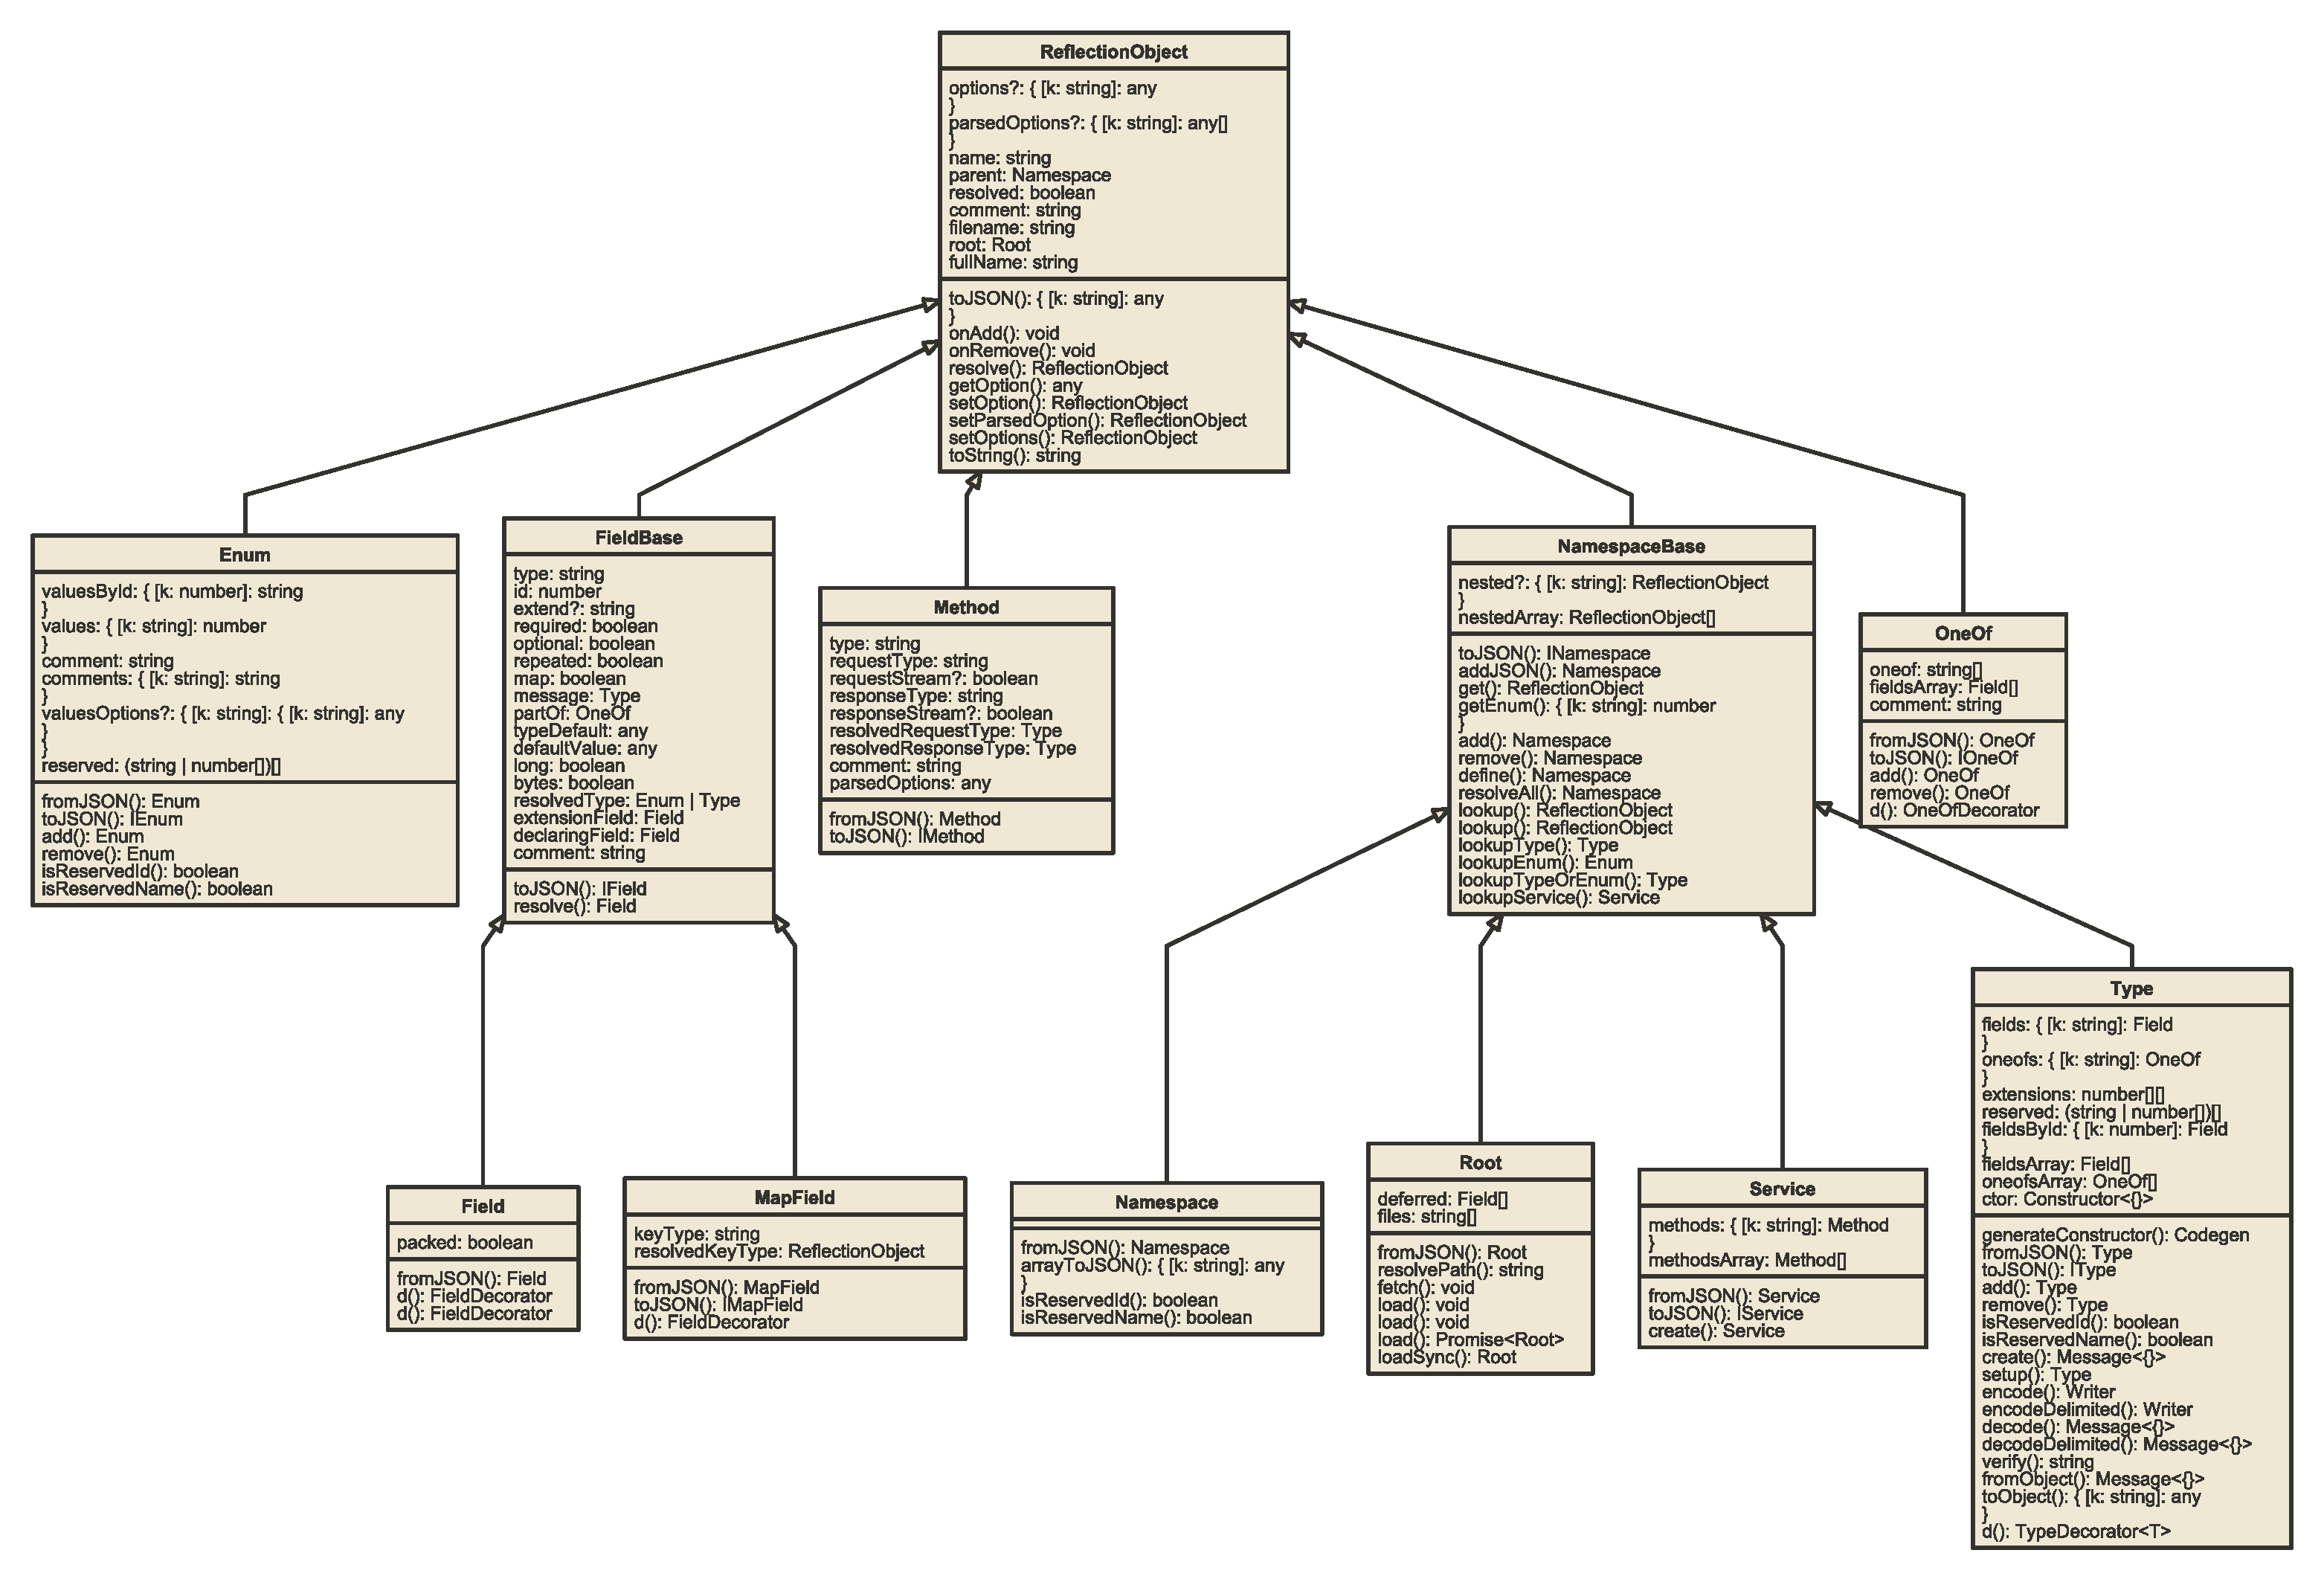
\includegraphics[width=0.75\paperheight]{images/implementation/protobufjs-class-diagram}
        \caption{Protobufjs class diagram~\cite{protobufjs}}
        \label{fig:protobufjs-class-diagram}
    \end{figure}
\end{landscape}

The base is the \textit{Root} class, which is returned by parsing the common format.
Other classes like service or type create a tree structure.
For example, using the field nested (or nestedArray) from the \textit{NamespaceBase}, I can traverse the tree and find all services, message types, or enums.
This way I find all the data I need for the website.

Each class has fields related to the protobuf features.
For example, the \textit{Service} class has a methods field, which contains all methods for that service, and the \textit{Method} class has a type or what type of streaming it is.
Also, all classes have a comment field which contains the comment from the proto file.
Using these fields, I can display the data on the website.

\subsection{User Interface}


\section{Licensing}
For the development, I have used libraries that use the following licenses:
\begin{itemize}
    \item MIT\footnote{\url{https://choosealicense.com/licenses/mit/}},
    \item BSD-3-Clause\footnote{\url{https://opensource.org/license/bsd-3-clause}},
    \item Apache 2.0\footnote{\url{https://choosealicense.com/licenses/apache-2.0/}},
    \item ISC\footnote{\url{https://www.isc.org/licenses/}},
    \item CC-BY-4.0\footnote{\url{https://creativecommons.org/licenses/by/4.0/}}.
\end{itemize}

The list of libraries and their licenses is captured in tables~\ref{tab:libraries-licenses} and~\ref{tab:libraries-licenses-dev}.
The rights and limitations of these licenses are then shown in table~\ref{tab:licenses}.

\begin{table}
    \centering
    \captionsetup{justification=centering}
    \begin{tabular}{|l|l|l|l|l|l|}
        \hline
        & \textbf{MIT} & \textbf{BSD-3-Clause} & \textbf{Apache 2.0} & \textbf{CC-BY-4.0} & \textbf{ISC} \\ \hline
        \textbf{Permissions}         &              &                       &                     &                    &              \\ \hline
        Commercial use               & \checkmark   & \checkmark            & \checkmark          & \checkmark         & \checkmark   \\ \hline
        Modification                 & \checkmark   & \checkmark            & \checkmark          & \checkmark         & \checkmark   \\ \hline
        Distribution                 & \checkmark   & \checkmark            & \checkmark          & \checkmark         & \checkmark   \\ \hline
        Patent use                   & -            & -                     & \checkmark          & x                  & -            \\ \hline
        Private use                  & \checkmark   & \checkmark            & \checkmark          & \checkmark         & \checkmark   \\ \hline
        &              &                       &                     &                    &              \\ \hline
        \textbf{Conditions}          &              &                       &                     &                    &              \\ \hline
        License and copyright notice & \checkmark   & \checkmark            & \checkmark          & \checkmark         & \checkmark   \\ \hline
        State changes                & -            & -                     & \checkmark          & \checkmark         & -            \\ \hline
        &              &                       &                     &                    &              \\ \hline
        \textbf{Limitations}         &              &                       &                     &                    &              \\ \hline
        Trademark use                & -            & -                     & x                   & x                  & -            \\ \hline
        Liability                    & x            & x                     & x                   & x                  & \checkmark   \\ \hline
        Warranty                     & x            & x                     & x                   & x                  & \checkmark   \\ \hline
    \end{tabular}
    \caption{Overview of licenses and their limitations}
    \label{tab:licenses}
\end{table}

All licenses allow both private and commercial use, including distribution and possible modifications.
The only requirement is to
%keep the license and copyright notice, eventually
state changes if made (I have not made any change to the libraries that require it).
% TODO Is it necessary to mention them somewhere in the project?
%All used libraries with their respective licenses can be found on the website


Because I have met the requirements of the licenses and their limitations allow me to use the libraries for free, I can use the libraries for my work.

\newcommand{\library}[1]{%
    #1\tablefootnote{\url{https://www.npmjs.com/package/#1}}%
}

\newpage
\begin{table}[hbt!]
    \centering
    \captionsetup{justification=centering}
    \begin{tabular}{|l|l|l|}
        \hline
        \textbf{Library}                              & \textbf{License} \\ \hline
        \library{@fortawesome/fontawesome-svg-core}   & MIT              \\ \hline
        \library{@fortawesome/free-regular-svg-icons} & CC-BY-4.0, MIT   \\ \hline
        \library{@fortawesome/free-solid-svg-icons}   & CC-BY-4.0, MIT   \\ \hline
        \library{@fortawesome/react-fontawesome}      & MIT              \\ \hline
        \library{@hookform/resolvers}                 & MIT              \\ \hline
        \library{bootstrap}                           & MIT              \\ \hline
        \library{grpc-web}                            & Apache-2.0       \\ \hline
        \library{lodash}                              & MIT              \\ \hline
        \library{next}                                & MIT              \\ \hline
        \library{p-cancelable}                        & MIT              \\ \hline
        \library{protobufjs}                          & BSD-3-Clause     \\ \hline
        \library{protobufjs-cli}                      & BSD-3-Clause     \\ \hline
        \library{react}                               & MIT              \\ \hline
        \library{react-bootstrap}                     & MIT              \\ \hline
        \library{react-dom}                           & MIT              \\ \hline
        \library{react-hook-form}                     & MIT              \\ \hline
        \library{react-syntax-highlighter}            & MIT              \\ \hline
        \library{sass}                                & MIT              \\ \hline
        \library{yup}                                 & MIT              \\ \hline
    \end{tabular}
    \caption{List of libraries and their licenses}
    \label{tab:libraries-licenses}
\end{table}

\newpage
\begin{table}[hbt!]
    \centering
    \captionsetup{justification=centering}
    \begin{tabular}{|l|l|l|}
        \hline
        \textbf{Development Library}              & \textbf{License} \\ \hline
        \library{@testing-library/jest-dom}       & MIT              \\ \hline
        \library{@testing-library/react}          & MIT              \\ \hline
        \library{@types/jest}                     & MIT              \\ \hline
        \library{@types/lodash}                   & MIT              \\ \hline
        \library{@types/node}                     & MIT              \\ \hline
        \library{@types/react}                    & MIT              \\ \hline
        \library{@types/react-dom}                & MIT              \\ \hline
        \library{@types/react-syntax-highlighter} & MIT              \\ \hline
        \library{cross-env}                       & MIT              \\ \hline
        \library{eslint}                          & MIT              \\ \hline
        \library{eslint-config-next}              & MIT              \\ \hline
        \library{eslint-config-prettier}          & MIT              \\ \hline
        \library{jest}                            & MIT              \\ \hline
        \library{jest-environment-jsdom}          & MIT              \\ \hline
        \library{prettier}                        & MIT              \\ \hline
        \library{typescript}                      & Apache-2.0       \\ \hline
        \library{lerna}                           & MIT              \\ \hline
        \library{rimraf}                          & ISC              \\ \hline
    \end{tabular}
    \caption{List of development libraries and their licenses}
    \label{tab:libraries-licenses-dev}
\end{table}